\chapter{\label{ch4-software}Software} 

\minitoc

\notes[inline,caption={}]{
	\section{Plan}
	\subsection{Topics}
	\begin{itemize}
		\item TargetIO/TargetDriver
		\item TargetCalib
		\item ctapipe
		\item gammapy/CTOOLS
	\end{itemize}
	\subsection{Questions}
	\begin{itemize}
		\item ?
	\end{itemize}
}

\section{Introduction}

In Chapter~\ref{ch3-architecture}, the data processing steps that are required in order to obtain the science data that is released by the \gls{cta} Observatory are described. In order to go from camera trigger to science results, a number of software packages must be developed, and be provided to \gls{cta} as in-kind contributions, as instructed by the \gls{cta} Architecture. 

This chapter provides an outline of the software packages used in the pipeline for \gls{chec} and \gls{cta}, alongside my contributions to them.

\section{TARGET Libraries}

A collection of libraries have been created to operate, readout, and calibrate the cameras containing \gls{target} modules (\gls{chec} and the \gls{sct} camera), and are therefore known as the ``TARGET Libraries''. These low-level libraries are wrote in \cpp as they prioritise efficiency over flexibility. To enable the use of these libraries from the Python packages used in waveform reduction, a Python wrapper for these libraries is automatically generated during compilation by \gls{swig}\footnote{http://www.swig.org/}.

These libraries are presently stored on the \gls{cta}-SVN version control server, and installation instructions can be found at \url{https://forge.in2p3.fr/projects/gct/wiki/Installing_CHEC_Software}, provided you have permissions to the \gls{gct} Redmine.

\subsection{\pkg{TargetDriver}}

In order to operate, or ``drive'', the \gls{target} modules, the \pkg{TargetDriver} library is required. This \cpp library configures the TARGET modules, and listens for the UDP packets containing the waveform data.

\subsection{\pkg{TargetIO}}

\begin{figure}
  \centering
  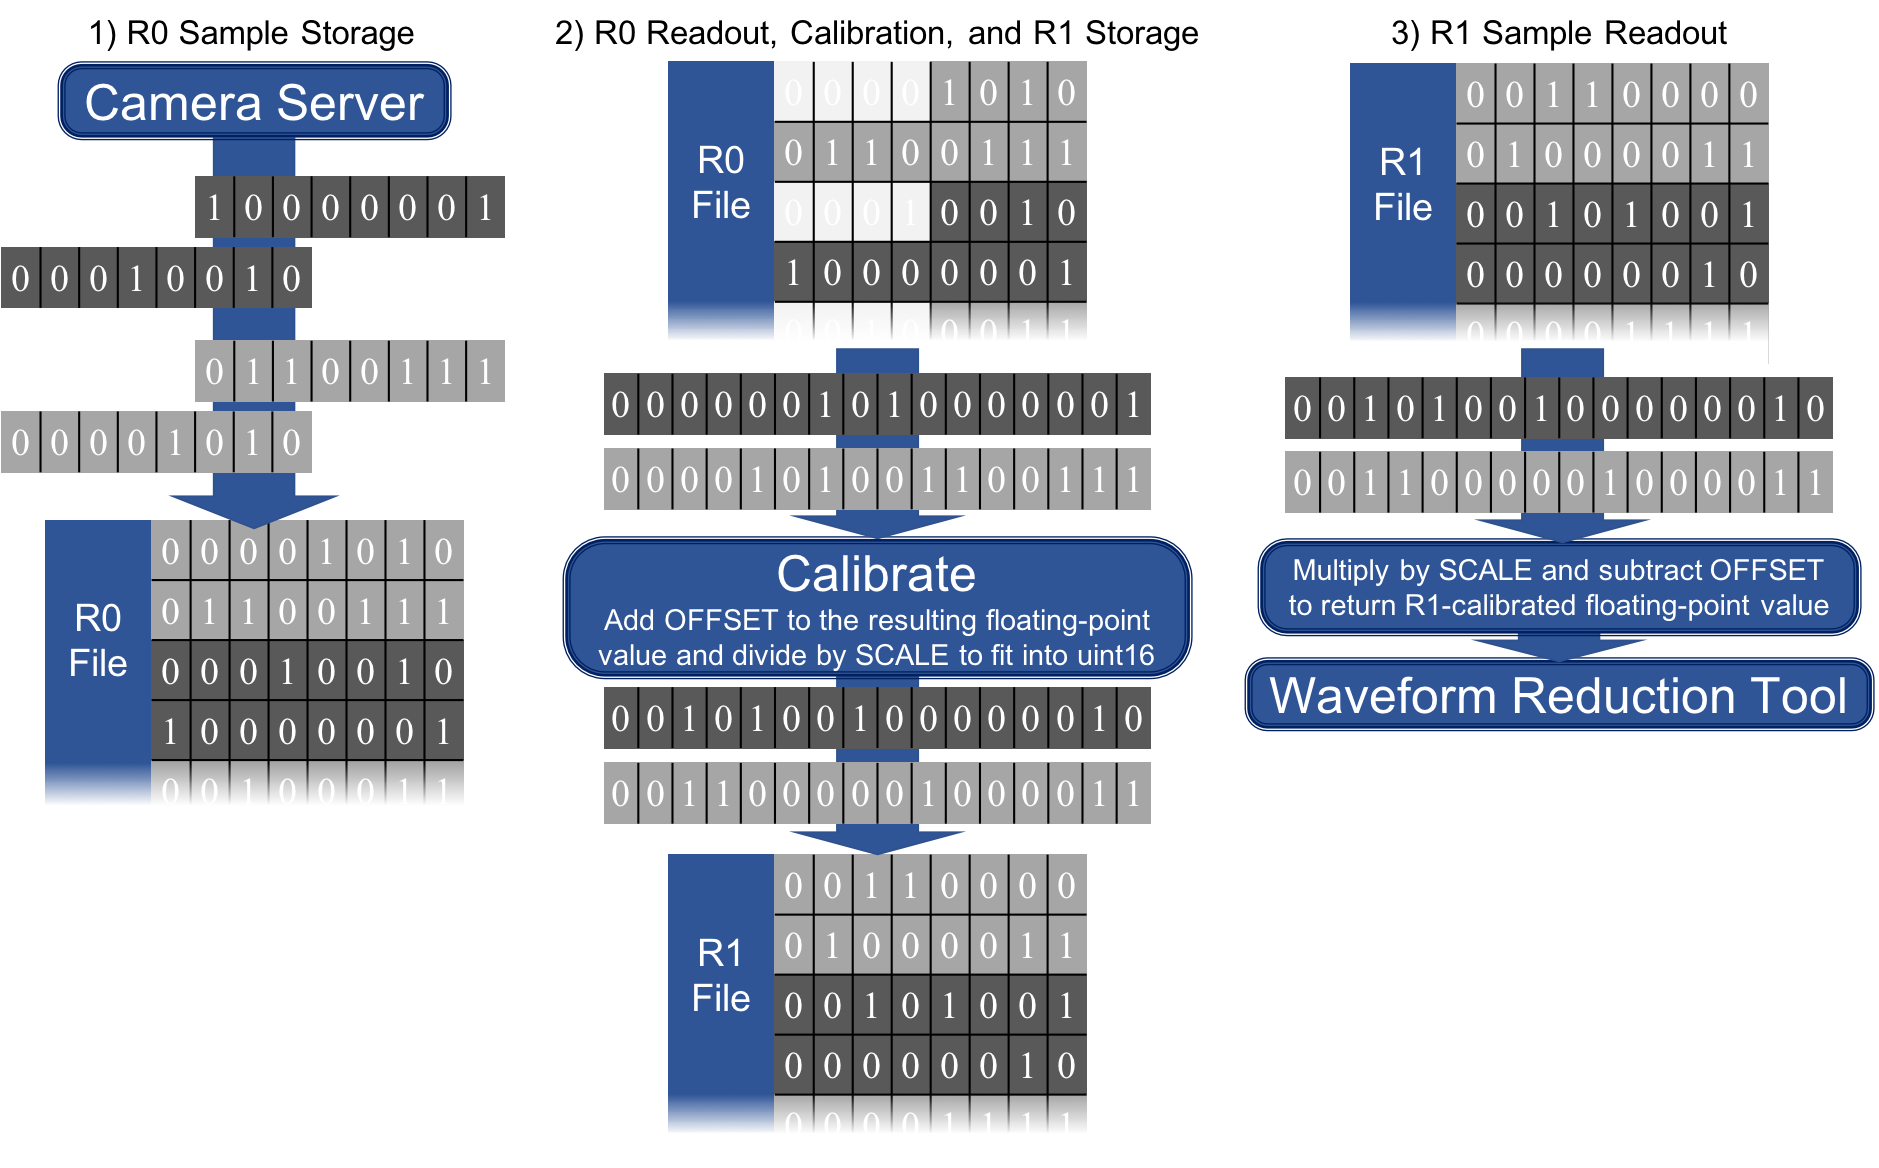
\includegraphics[width=\textwidth]{figures/images/tio}
  \captionsetup{singlelinecheck=off}
  \caption[Simple overview of the data-flow for waveform samples within the TARGET libraries]{Simple overview of the data-flow for waveform samples within the TARGET libraries:
  \begin{enumerate}[label={\arabic*)}]
  \item 8-bit/char packets are sent from the TARGET FPGA and stored directly to file. A waveform sample is 12-bit, therefore the first four bits of the first 8-bit sample packet are used to indicate sample order.
  \item When reading a sample from the R0 TIO file, the first four bits are ignored, and the remaining twelve bits are combined into an unsigned 16-bit sample. The samples are passed to \pkg{TargetCalib} for calibration. The resulting calibrated floating-point sample is scaled and offset to fit into an unsigned 16-bit integer for storage.
  \item When reading a sample from a R1 TIO file, the entirety of the two 8-bit packets are kept and combined. The value is returned to floating-point format using the OFFSET and SCALE stored in the file header.
  \end{enumerate}
  
  Although only the samples are shown here, all other waveform data is also sent along this stream, including ASIC and Channel number, indicating the start of a new waveform. 
  }
  \label{fig:tio}
\end{figure}

The file format used to store waveforms from \gls{target} modules is a custom \gls{fits} format defined by \pkg{TargetIO}, hereby referred to as the \gls{tio} format. This library is always used to read and write waveform and header (information such as observation time) data to the \gls{tio} file. \gls{tio} files can either contain \textit{R0} (uncalibrated)  or \textit{R1} (low-level calibrated) waveform data. Each sample in a waveform is stored to file as an unsigned 16-bit integer. The raw waveform digital counts measured by the camera are serialised in an unsigned 12-bit integer format, and the data packets received from the \gls{target} \gls{fpga} are 8-bit in size, therefore the first 4 bits of a waveform sample inside an \textit{R0} \gls{tio} file are not used. When storing calibrated waveforms, the post-calibration floating-point sample is scaled and offset to fit the full 16-bit unsigned integer. These scale and offset values are stored in the file header and automatically applied to convert the sample back into floating-point format when read. Figure~\ref{fig:tio} demonstrates the data-flow processes involving the \gls{tio} files.

To ensure the full efficiency of the \cpp library is exploited via the Python wrapper, I contributed the |WaveformArrayReader| class, which, when passed a contiguous block of memory (such as a \lstset{language=Python}|numpy.array|), promptly fills the array with the entire camera's waveform data for that event. For example, to read an \textit{R1} \gls{tio} file from Python:

\begin{lstlisting}[language=Python]
import numpy as np
from target_io import WaveformArrayReader

# Create the reader and get the number of pixels and number of samples from the header
reader = WaveformArrayReader("/path/to/file/Run17473_r1.tio")
n_pixels = reader.fNPixels
n_samples = reader.fNSamples

# Generate the memory to be filled in-place
waveforms = np.zeros((n_pixels, n_samples), dtype=np.float32)
first_cell_ids = np.zeros(n_pixels, dtype=np.uint16)  # Storage cell id for the first sample of the event per pixel

# Fill the arrays
event_index = 20
reader.GetR1Event(event_index, waveforms, first_cell_ids)
# `waveforms' array is now filled with entire event's waveform data
\end{lstlisting}

\subsection{\pkg{TargetCalib}}

To correct for the effects of the \gls{target} electronics on the waveforms, \pkg{TargetCalib} was built. I have led the development of this package since its early development. The calibrations performed by this library are detailed in Chapter~\ref{ch5-calibration}. This package has also been adopted by \gls{sct} recently.

The main classes in the library include:

\lstset{language=C++}
\begin{description}
\item [\textbf{PedestalMaker}] Generates the \textit{Pedestal} calibration file.
\item [\textbf{TfMaker}] Generates the \textit{Transfer Function} calibration file.
\item [\textbf{Calibrator}] Applies the aforementioned calibration files to the waveform samples.
\item [\textbf{Mapping}] Handles the files containing the camera's pixel mapping, and provides an interface to the information. This class is necessary due to the non-intuitive mapping between physics pixel position, and order of pixel readout (Figure~\change{figure showing the pixel positions, camera or module?}). Most commonly, this mapping is used for the plotting of camera images. The class is compatible with the mapping of any square-pixel telescope, and customisable to provide the mapping of the pixels in a single module, the mapping of the superpixels, the mapping of the modules, or the neighbours to a pixel/superpixel/module. This class will be deprecated once the central \gls{cta} database of telescope configurations exists.
\item [\textbf{CameraConfiguration}] Provides an interface to certain camera-version dependant variables. Currently the variables that might change with camera-version (stored in the \gls{tio} file header) include number of storage cells, pixel mapping, and reference pulse shape. The correct version of the parameter is returned according to the camera-version provided, allowing for the automated processing of the data of different camera versions. This class will also be replaced by the central \gls{cta} database.
\end{description}

Efforts are being made to improve the \pkg{TargetCalib}'s (more specifically the |Calibrator| class's) efficiency in terms of both memory and processing time, as it will need to meet the \gls{cta} Requirements for \textit{Online Analysis} (Chapter~\ref{ch3-architecture}). It is possible that in the future there will be two separate |Calibrator| classes for the \textit{Online} and \textit{Offline Analyses} respectively.

\section{Reduction Tools}

Tools used to process the waveforms in order to either characterise the camera or progress down the data-level-chain (Figure~\ref{fig:dataflow}) are often referred to as ``reduction tools''. Within the \gls{chec} group we utilise Python for all of our waveform reduction. We made this choice due to its high popularity for data science and signal processing and its extensive library of statistical and numerical packages. The most important examples of these packages include:

\begin{description}
\item [\textbf{NumPy\footnotemark}] \footnotetext{http://www.numpy.org/} Enables the efficient processing of numerical data. This is accomplished using their powerful N-dimensional array object known as a |numpy.array|. At the lowest level, a |numpy.array| is a contiguous block of memory much like a C array. However, NumPy defines many statistical methods which utilise optimised low-level C and Fortran operations to process the contained data in the most efficient way possible, often performing better than handwritten C or Fortran.
\end{description}

Different reduction packages may be designed with different purposes, but each can potentially import methods from another, which is especially possible when developing in Python. Many other \gls{cta} groups have also adopted Python for their waveform reduction software, but it is not a standard across \gls{cta}.

\subsection{\pkg{ctapipe}}

\subsection{\pkg{CHECLabPy}}

\section{Science Tools}

\subsection{\pkg{GammaPy}}

\subsection{\pkg{CTOOLS}}